\chapter[Estruturação e Implementação da Gamificação da About]{Estruturação e Implementação da Gamificação da About}
Para a implementação do trabalho, os seguintes
passos foram executados, cada um é
descrito em uma subseção: execução do teste piloto, \textit{survey} para identificação das técnicas de Gamificação,
análise estatística das técnicas, construção do \textit{framework} de Gamificação, escolha do objeto de Gamificação,
implementação das técnicas no objeto de Gamificação.
Aqui serão relatados todos os passos que foram tomados para a realização do trabalho.

\section{Execução do Piloto}
\label{sec:execucao_do_piloto}
Com a intenção de validar a aplicação da About, foi implementado um piloto com as suas funcionalidades
básicas. Aqui existia apenas um post, onde o administrador da aplicação escolhe dentre temas propostos
pelos usuários, que era postado a cada três dias.
Nesta sessão iremos descrever sobre como esta implementação foi executada.

Para desenvolver e aplicar este piloto, será necessário executar um procedimento
com os seguintes passos:

\begin{enumerate}
    \item Definir tecnologia;
    \item Desenvolver solução;
    \item Implantação em produção;
    \item Aplicar \textit{marketing} da solução para um público reduzido;
    \item Manter solução;
    \item Finalizar solução.
\end{enumerate}


Primeiramente, haviam alguns pontos necessários para a implantação da aplicação. 
Assim como ter agilidade para desenvolvê-la e colocá-la em produção.
Estes foram os padrões seguidos para a produção do piloto:


\begin{itemize}
    \item Desenvolvimento rápido;
    \item Padrões de \textit{design} simples;
    \item Escalabilidade baixa;
    \item Os usuários não carecem de executar cadastros e logins;
    \item Suporte para questionários;
    \item Facilidade de implantação.
\end{itemize}

Todos estes pontos foram avaliados. Desta forma, era necessário implementar um \textit{software}
de alta produtividade, que entregasse a funcionalidade muito rapidamente. Assim, dados estes
pontos, a tecnologia escolhida foi o WordPress, utilizando a linguagem de programação PHP.

Um \textit{software} desenvolvido utilizando WordPress possui vários módulos prontos, mantidos pela comunidade e fornecidos de maneira
gratuita. Nestes módulos, temos componentes para questionários, com \textit{designs} padronizados,
implementados e de extrema facilidade de utilização.

Como o \textit{software} é considerado pequeno, não houve nenhuma necessidade de preocupação com a
infraestrutura  do sistema e com fatores técnicos ligados à alta performance. Também não foi
necessário fazer um controle de acessos e de usuários, pois a votação seria baseada no IP
do cliente, não permitindo novos acessos daquele mesmo IP.

Escolhida a tecnologia, foi iniciada a implementação da aplicação. Esta consistiu em escolher o
módulo de enquete e o módulo de \textit{layout}. Após isto, tudo estava finalizado.

Para enquetes, foi
utilizado o pacote WP-Polls, este pode ser encontrado em: \url{https://wordpress.org/plugins/wp-polls/}.

Para a implementação do \textit{layout} foi utilizado o módulo Amadeus, que pode ser encontrado em:
\url{https://br.wordpress.org/themes/amadeus/}.

No âmbito da implantação foi necessário apenas comprar um servidor cloud e instalar os pacotes do WordPress
dentro deste. O código fonte da aplicação pode ser encontrado neste link:
\url{https://wordpress.org/download/}.

Implementada a solução e operando, foi necessário divulgá-la para aqueles que utilizariam o código.
Então foi criado um perfil na rede social \textit{Facebook}, onde foi divulgado para todos os alunos de engenharia
de \textit{software} o propósito do site, assim como cada um poderia utilizá-lo. Dessa forma, foram feitas postagens diárias
na página falando sobre as notícias da aplicação. A comunidade em si se empolgou bastante com os novos resultados.

O perfil ganhou vários seguidores que participavam ativamente ou passivamente da plataforma, respondendo, criando e
visualizando os posts realizados no projeto piloto.

Para manter a solução, era necessário levantar enquetes para o público. Então, para manter o público interessado,
foi criado uma segunda enquete que sempre estava disponível perguntando aos usuários:

Qual tema vocês desejam ver no próximo post piloto?

Assim, todos os temas mais pedidos pelo público eram lançados e mantidos ao longo de dois dias para uma votação.

Por fim, foi declarado que seria finalizada a solução e que o último post seria feito. Este foi realizado para a
última votação. E assim o piloto saiu de produção.

\section{Levantamento das Técnicas de Gamificação}
\label{sec:implementacao_levantamento}
Com base em uma pesquisa executada com os participantes do piloto, foi executado um levantamento das
técnicas básicas, para colocá-las frente aos objetivos estabelecidos no trabalho.

Primeiramente foi perguntado a alguns usuários que utilizaram a rede social quais impressões estes tiveram
do software utilizado.
Claro que o intuito de todas as perguntas era identificar como os usuários visualizavam dinâmicas
que envolviam Gamificação dentro do piloto.

As perguntas realizadas aos usuários foram as seguintes:

\begin{quotation}
    Questão 01: Na sua opinião, o que este \textit{site} representava?
\end{quotation}

\begin{quotation}
    Questão 02: O que você acredita que motivava e levava as pessoas a utilizarem o \textit{site}?
\end{quotation}

\begin{quotation}
    Questão 03: E quanto ao contrário, o que você acredita que levava as pessoas a se desmotivarem e a não
    utilizarem mais o \textit{site}?
\end{quotation}

Assim, para estas perguntas, tivemos um total de 4 pessoas respondendo este questionário.
As etapas foram divididas em questões, listando assim suas respectivas respostas. 
A resposta de cada usuário será descrita a seguir.

\subsection{Questão 01}
\subsubsection{Usuário 01}
A curiosidade levava as pessoas a entrarem na plataforma e descobrirem o que as
pessoas estavam falando das outras.
\subsubsection{Usuário 02}
Era uma oportunidade de trazer a tona todos os sentimentos e sensações das pessoas
em relação as outras. Tanto relação a atitudes quanto a impressões sobre eventos
passados. Uma oportunidade de trazer visibilidade para a consequência de uma ação
feita por alguém.
\subsubsection{Usuário 03}
Criatividade.
\subsubsection{Usuário 04}
Um site que surgiu na faculdade, que a princípio era um portal para relatos de
acontecimentos da faculdade UnB-FGA, onde existiam vários posts inimagináveis
de algumas pessoas. E era confirmado este relato quando você via os outros comentários
anônimos, reforçando exatamente aquele ponto. Eram comentários que a princípio ninguém
acreditaria, pois eram extremamente fortes. Chegando a chocar com os fatos
declarados.

\subsection{Questão 02}
\subsubsection{Usuário 01}
A curiosidade das pessoas em relação aos segredos de outras que não são contados no cotidiano.
\subsubsection{Usuário 02}
Oportunidade de punir atitudes/ações consideradas erradas pelos usuários do site. Mostrando que há consequências para pessoas que publicam conteúdos de natureza ofensiva, e que elas serão expostas ao fazer algo de ruim para o meio.
\subsubsection{Usuário 03}
Curiosidade.
\subsubsection{Usuário 04}
Você não quer ser um alvo do post da plataforma, você quer ser aquele que julga.
Então criava-se a curiosidade sobre os comentários feitos à minha pessoa e também
os comentários feitos a outras pessoas. 
A rede era estimulada pelo ambiente de "fofoca".

\subsection{Questão 03}
\subsubsection{Usuário 01}
Medo de exposição de seus detalhes pessoais para demais indivíduos.
\subsubsection{Usuário 02}
A probabilidade de perder o controle diante da invasão de privacidade. E trazer
consequências reais para a vida da pessoa.
\subsubsection{Usuário 03}
Falta de atualizações e novos conteúdos para o portal, deixando-o mostrar apenas mais do mesmo.
\subsubsection{Usuário 04}
Medo de que seu nome estivesse ali no meio da plataforma e a falta de existência
de um meio de defesa para os acusados.

Terminadas as perguntas aos usuários, evidencia-se que para todos a maior motivação era curiosidade, o desejo de saber sobre o desconhecido. Logo, já é possível notar a presença de algumas motivações básicas de Gamificação relacionadas a curiosidade.

\subsection{Conclusão do Questionário}
Mas ainda assim, esta análise qualitativa não mostrou muito sobre quais fatores
e quais motivações básicas de fato eram percebidas no piloto executado. Assim,
como planejado, foi executado um \textit{survey}, para obter resultados quantitativos sobre
o quanto cada técnica estava influenciando o procedimento de Gamificação dentro
daquela aplicação. Estes passos serão descritos na próxima sessão.

\section{Survey das Técnicas}
\label{sec:gamifição}
Para apurar as técnicas capturadas no levantamento, foi executado um \textit{survey}, a fim de dados para
embasar uma análise estatística.

Para este \textit{survey}, foi utilizada uma escala de 0 a 5. Assim, foram apresentadas aos usuários
que fizeram o primeiro levantamento todas as técnicas de Gamificação, com a sua
respectiva explicação. O usuário deveria votar e dizer o quanto cada técnica estava presente
dentro do escopo do piloto. As técnicas utilizadas são as apresentadas na sessão
\ref{sub:an_lise_estat_stica_das_t_cnicas}.

Primeiramente, para entender qual o perfil do entrevistado no trabalho, foi elaborado
um questionário prévio para traçar seus aspectos pessoais,
para que pudesse ser entendido qual a relação que esse tem com jogos e com dinâmicas
voltados à Gamificação. Todos estes podem ser vistos neste \href{https://docs.google.com/spreadsheets/d/1galTU00NPQKaU7GRsYOciLhD0ZzIKH9BbJWyRdC3gbs/edit?usp=sharing}{link}.

Para a elaboração da enquete, foi apresentado um formulário a cada usuário, solicitando
que este votasse em todas as técnicas. A tabela com o resultado está neste
\href{https://docs.google.com/spreadsheets/d/1qROpsDaz32PZtkvCvmFTrqLVLgqhHR9F-Q5rcQ_pwys/edit?usp=sharing}{link}.

A partir de todos estes dados, foi possível executar os cálculos da sessão \ref{sub:implementa_o_das_t_cnicas}
e montar o \textit{Framework}, como apresentado no exemplo da figura \ref{fig:exoctalysis}.

Antes de executar o cálculo, foi elaborada a Tabela \ref{tab:percentual_tecnica_motivacao}
 de notas, onde é possível
observar a quantidade total possível e a quantidade de pontos feita por cada técnica.
Bem como a porcentagem que esta representa.

\begin{table}[]
    \centering
    \caption{Percentual de Técnica por Motivação Básica}
    \label{tab:percentual_tecnica_motivacao}
    \begin{tabular}{@{}cccc@{}}
        \toprule
        Motivação Básica & Pontos de Votos & Pontos Totais & Percentual \\ \midrule
        1         & 68            & 140             & 48,57\%    \\
        2         & 102           & 280             & 36,43\%    \\
        3         & 62            & 160             & 38,75\%    \\
        4         & 38            & 120             & 31,67\%    \\
        5         & 93            & 200             & 46,50\%    \\
        6         & 20            & 100             & 20,00\%    \\
        7         & 74            & 120             & 61,67\%    \\
        8         & 32            & 60              & 53,33\%    \\ \bottomrule
    \end{tabular}
\end{table}

Executada esta tabela, já seria possível criar o \textit{Framework} de Gamificação. Assim,
este finalizado pode ser visto na Figura.

\begin{figure}[h]
    \centering

    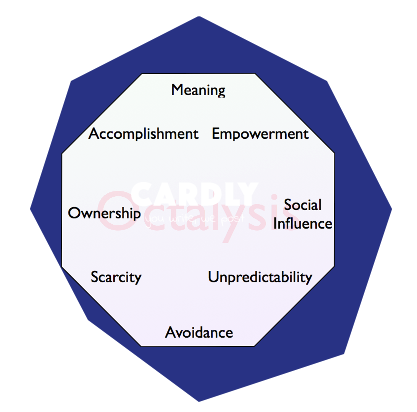
\includegraphics[width=250px, scale=1]{figuras/final_survey}
    \caption{\textit{Framework} final do \textit{Survey}}

    \label{fig:final_framework_octalisys}
\end{figure}

Assim, como todos estes dados, é possível iniciar um procedimento de estudo de Dados.
Todas essas análises serão feitas na próxima sessão.

\section{Análise Estatística}
\label{sec:implementacao_analise_estatistica}
Com base nos dados obtidos no \textit{survey}, foram definidas quais as técnicas tem relação entre si para auxiliar no processo
de escolha para o \textit{framework}.

Todos estes estudos com base nos dados foram feitos através do resultado do \textit{survey} aplicado nos usuários
da plataforma. Estes foram armazenados em uma planilha ODS.

Para fazer todas essas análises, foi necessário escolher uma ferramenta de processamento de dados.

Como a ferramenta escolhida foi a RScript, da sessão 4.4.1, iremos proceder todos os detalhes de implementação
levando em consideração essa tecnologia.

Assim, foi feita a instalação dos pacotes. Dessa forma foi  analisado
se este está instalado dentro da máquina. 
Caso esteja, o projeto vai continuar o código contrário, estes serão instalados.

\lstinputlisting[language=Python, firstline=3, lastline=10]{statistics.r}

Assim que a aplicação certifica que todos estão instalados, estes são carregados
para a aplicação da seguinte maneira:

\lstinputlisting[language=Python, firstline=12, lastline=19]{statistics.r}

Carregados todos os módulos, iniciamos em um processo de leitura da tabela ODS.
Existe uma lib na linguagem RScript para parser deste tipo de arquivo, convertendo
para dados estruturados em listas e arrays. Estes códigos podem ser vistos a seguir:

\lstinputlisting[language=Python, firstline=21, lastline=23]{statistics.r}

O algorítimo de processamento dos dados retorna um valor errado caso tenha alguma
linha de dados sem valor de votação. Assim, para resolver esses erros, foram eliminadas
todas as linhas que possuem este tipo de valor. Este processamento pode ser visto nos
comandos a seguir:

\lstinputlisting[language=Python, firstline=25, lastline=26]{statistics.r}

Agora com todos os dados tratados e prontos dentro do algorítimo, alguns cálculos podem
ser executados. Primeiramente, será criado o Alpha de Cronbach. Para isso, iremos utilizar
a lib Alpha. 

\lstinputlisting[language=Python, firstline=28, lastline=29]{statistics.r}

Dado que o Alpha foi calculado, podemos gravar em disco os três tipos de saída que são geradas.
A primeira delas é o cálculo para cada item separadamente. A segunda se trata da média destes
itens. Por fim, temos os cabeçalhos e detalhes relativos a todo o cálculo. Todos esses dados serão
salvos em disco em arquivos diferentes. 

\lstinputlisting[language=Python, firstline=31, lastline=38]{statistics.r}

Agora, será executado o resultado do algorítimo da correlação de Pearson, utilizando
também a tabela de votos sem os valores inválidos. Em seguida, este também foi salvo em disco
com um arquivo CSV.

\lstinputlisting[language=Python, firstline=40, lastline=45]{statistics.r}

Realizado todos estes passos, podemos então trabalhar com os dados executados.
Assim, foi executada uma sumarização dos dados para facilitar a visualização destes.
Sendo logo colocados em uma planilha CSV. Este código está disposto a seguir:

\lstinputlisting[language=Python, firstline=47, lastline=49]{statistics.r}

Para que fosse executada a aplicação do algorítimo Apriori, foi necessário fazer
algumas transformações nas operações. Entre estas estavam:

\begin{itemize}
    \item Fazer a conversão da tabela em uma matriz;
    \item Transformar valores acima de 4 em unidades binárias ligadas;
    \item Transformar valores abaixo de 4 em unidades binárias desligadas;
    \item Transformar a matriz modificada em transactions;
    \item Criar as rules utilizando o Apriori.
\end{itemize}

\lstinputlisting[language=Python, firstline=51, lastline=81]{statistics.r}

Finalizados os apuramentos de dados, foi possível analisar quais técnicas tem correlação
entre si, possibilitando assim uma orientação para a escolha de quais técnicas se interligam
e que podem vir a ser importantes para implementar na rede social About. A construção
do \textit{Framework} será apresentada no próximo capítulo.

\subsection{Resultados do Algorítimo}
Quanto ao resultado dos algorítimos, todos eles estão armazenados em um repositório publicamente
para acesso. 

Aqui estão todos os resultados finais. Um resumo das técnicas que foram utilizadas pelo Framework final.
Está o batimento de todas as correlações das técnicas: 
\url{https://github.com/TiagoAssuncao/tcc-r/blob/master/table.ods}

Aqui é possível observar o resumo do Alpha, contendo os valores médios de todo o cálculo:
\url{https://github.com/TiagoAssuncao/tcc-r/blob/master/bin/alpha.csv}

Logo em seguida, é possível observar a média de cada item do Alpha:
\url{https://github.com/TiagoAssuncao/tcc-r/blob/master/bin/alpha_averange.csv}

Por fim, temos os resultados da correlação de Pearson:
\url{https://github.com/TiagoAssuncao/tcc-r/blob/master/bin/pearson.csv}

\section{Construção do \textit{Framework}}
\label{sec:gamifição}
Definidas as técnicas para a implementação, estas foram utilizadas para a construção do \textit{Framework}
de Gamificação.

Desta maneira, o \textit{Framework} final de Gamificação foi estabelecido e pode ser visto
na figura \ref{fig:final_project_octalisys}, para executar a implementação
deste. Com a visualização dos dados analisados da sessão \ref{sec:implementacao_analise_estatistica}
e dos dados relatados pelos usuários na sessão, \ref{sec:implementacao_levantamento}, o seguinte \textit{Framework}
foi construído:

\begin{figure}[h]
    \centering

    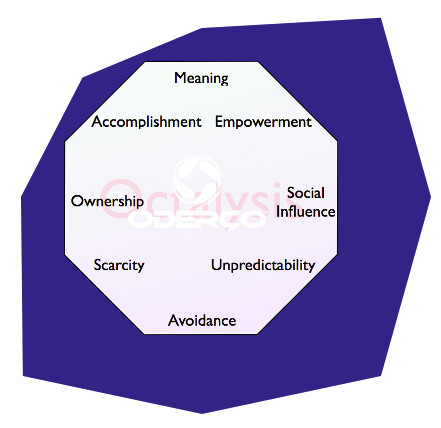
\includegraphics[width=250px, scale=1]{figuras/final_framework}
    \caption{\textit{Framework} final do Projeto}

    \label{fig:final_project_octalisys}
\end{figure}

Todas estas técnicas serão aplicadas nos objetos de Gamificação que  serão definidos na próxima sessão.

\section{Objeto de Gamificação}
\label{sec:implementacao_objeto_gamificao}
Assim que todo o \textit{Framework} foi montado, possibilitou então que fossem escolhidos em quais
pontos da About seria possível aplicá-los. Esta sessão irá discutir sobre todos os pontos de escolha
dos objetos de Gamificação.

Como são várias técnicas de diferentes motivações básicas, esta sessão será dividida em subseções, onde
cada uma trará todas as decisões destes objetos de Gamificação. Assim, o procedimento será divido entre
as seguintes motivações: Empoderamento e \textit{Feedback}, Influência Social, Imprevisibilidade,
Escassez e para finalizar,  Perda e Rejeição.

\subsection{Objeto para Empoderamento e \textit{Feedback}}
\label{sub:objeto_empoderamento_feedback}
O motivação básica, Empoderamento e \textit{Feedback}, foi implementada dentro da rede social About, para apresentar
ao usuário maneiras de que esse tivesse \textit{feedback} sobre a impressão que toda a rede
tem do seu perfil. As técnicas utilizadas para tal implementação foram as seguintes:

\begin{itemize}
    \item \textit{Instant} \textit{Feedback};
    \item \textit{Foice} \textit{Perception}.
\end{itemize}

Com essas técnicas, o usuário da base conseguirá ter de outros usuários \textit{feedbacks},
utilizando assim os abouts já escritos.

Esta motivação é importante e será aplicada nas fases de entrada e dia a dia do usuário.

\subsection{Objeto para Influência Social}
\label{sub:objeto_influencia_social}
Na rede social About, há a necessidade de que os usuários tenham relação e influência
social entre si. Este valor emocional liga os usuários e os mantém engajados para utilizar
a plataforma. Desta maneira, as seguintes técnicas foram levantadas para esta motivação
básica:

\begin{itemize}
    \item Prateleira de Troféus;
    \item Orgulho Social;
    \item Tesouro Social.
\end{itemize}

Estas técnicas foram implementadas para apresentar ao usuário diferentes meios de interação
social, bem como votar em um dado About, comentá-lo, ter troféus por abouts escritos e julgados. 
E além disso, ser apresentado aos usuários aumenta esta influência.

Esta motivação é muito importante para que o usuário se mantenha na rede social. Ela será aplicada
na fase do dia a dia do usuário.

\subsection{Objeto para Desenvolvimento e Realização}
\label{sub:objeto_desenvolvimento_e_realizacao}
Para a motivação de Desenvolvimento e Realização é extremamente importante  que o usuário acompanhe seu progresso
na obtenção de pontos. Para isto, as seguintes técnicas foram utilizadas:

\begin{itemize}
    \item Pontos;
    \item Barra de Progresso.
\end{itemize}

Esta motivação será aplicada na fase do dia a dia do usuário, motivando-o a sempre subir de nível
e conseguir pontos suficientes para liberar as suas metas.

\subsection{Objeto Imprevisibilidade \& Escassez}
\label{sub:objeto_imprevisibilidade}
Estas duas motivações básicas - Imprevisibilidade \& Escassez -,  já estão implementadas na Rede Social About pela sua essência e foi
decidido não aplicar outras técnicas, pois estas motivações já tem técnicas suficientes implementadas.

O fato do usuário nunca saber quem irá elaborar um dado About ou quem irá votar lhe dá
todos os atributos de imprevisibilidade. 

Já para quem está de fora da rede social About e vê apenas alguns abouts sendo escritos, é uma forma
de ligar a escassez de não poder ler estes e assim gerar a curiosidade.

Estas duas técnicas são fundamentais para a entrada do usuário na rede social. E será implementada
nas fases de Descoberta e Entrada.

\subsection{Objeto para Perda e Rejeição}
\label{sub:objeto_perda_rejeicao}
A Perda e Rejeição foi utilizada como parte importante do projeto para motivar o usuário a não deixar a rede
social e sempre estar atualizando e participando. Para esta motivação, foi implementada a seguinte técnica:

\begin{itemize}
    \item \textit{FOMO} \textit{Ponch}.
\end{itemize}

A \textit{FOMO} \textit{Ponch} foi utilizada como forma do usuário perder pontos na rede social caso não escreva um About para alguém
dentro de um determinado período de tempo. Assim, a cada dia consecutivo que este está ativo
, ele ganha pontos ao escrever abouts. Caso passe um dia sem escrever, a sua pontuação volta ao início, adicionando
poucos pontos a cada About criado.

Esta motivação será aplicada na fase de fim de jogo do usuário, motivando-o a sempre entrar na plataforma
e a não deixar de escrever abouts.

\section{Implementação das Técnicas}
\label{sec:gamifição}
Assim que todo o \textit{Framework} foi estabelecido e seus objetos também, foi possível implementar
na rede social todos os pontos para colocar estas técnicas em prática.

As técnicas implementadas na rede social serão apresentadas na mesma ordem da sessão
\ref{sec:implementacao_objeto_gamificao}, mostrando os detalhes de utilização do usuário dentro
da motivação básica.

\subsection{Implementação para Empoderamento e \textit{Feedback}}
\label{sub:implementacao_empoderamento_feedback}
Para a implementação Empoderamento e \textit{Feedback}, foi implementado um meio que o usuário conseguisse
saber dos demais companheiros impressões sobre seus abouts, tendo \textit{feedbacks} sobre, em consequência,
da sua personalidade. 

Assim, foi criado um novo ambiente, onde um usuário visualiza cinco abouts de um outro usuário
da sua rede de amigos escolhido aleatoriamente. Após ler todos os abouts, ele escreve um \textit{feedback}, 
que aparecerá para o receptor como outro About. Aqui o usuário tem \textit{feedback} instantâneo sobre
sua impressão de vários usuários. 

O Empoderamento e \textit{Feedback}  será responsável por trabalhar no engajamento do usuário entre a
fase de entrada e a do dia a dia, assim que ele começa a utilizar a rede social e já possui
alguns poucos abouts. 

Além disso, os próprios abouts são maneiras de \textit{feedback} sobre a personalidade em questão, o
que contribui mais uma vez para a execução desta técnica.

A seguir, na figura \ref{fig:julgamento_menu}, está a indicação da técnica que foi batizada de Julgamento. Pois ali o juiz
irá dar uma impressão sobre vários usuários.

\begin{figure}[h]
    \centering
    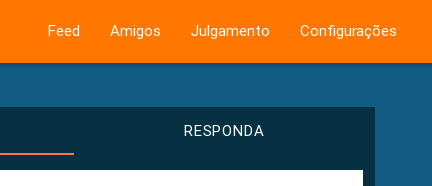
\includegraphics[width=250px, scale=1]{figuras/julgamento_menu}
    \caption{Menu com o Julgamento}
    \label{fig:julgamento_menu}
\end{figure}

Na figura \ref{fig:julgamento} será apresentado o formato de dados para o usuário teste,
criado pela biblioteca do \textit{Facebook} JoeAlbbfibifihjdSeligsteinse.

\begin{figure}[h]
    \centering
    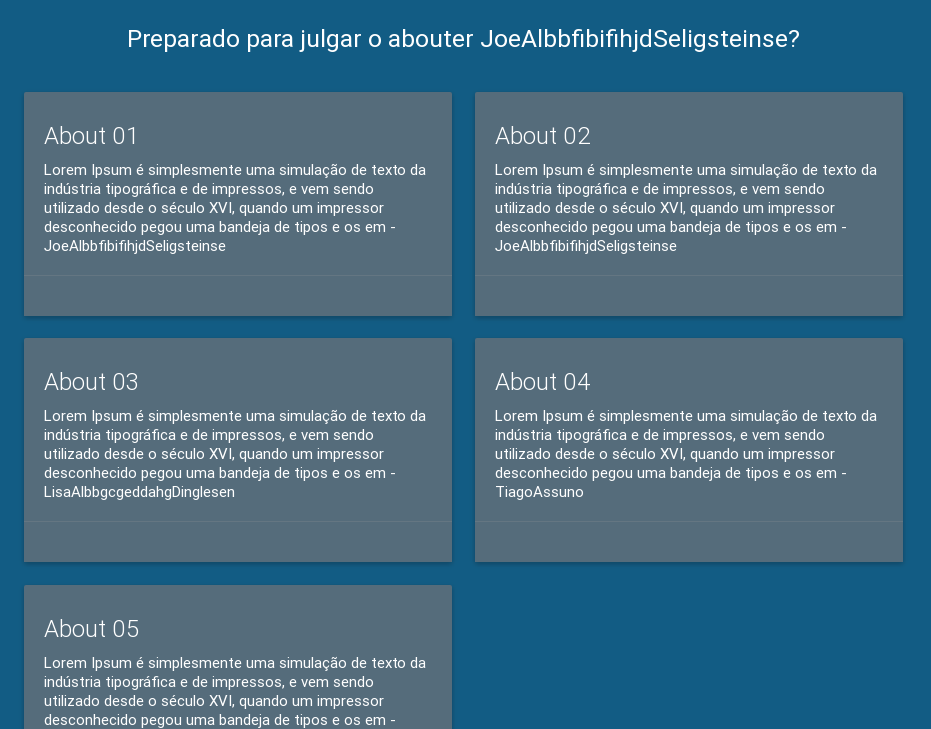
\includegraphics[width=350px, scale=1]{figuras/julgamento}
    \caption{Julgamento}
    \label{fig:julgamento}
\end{figure}

E logo abaixo, existe o campo para o usuário executar o julgamento, na figura \ref{fig:julgamento_about}.

\begin{figure}[h]
    \centering
    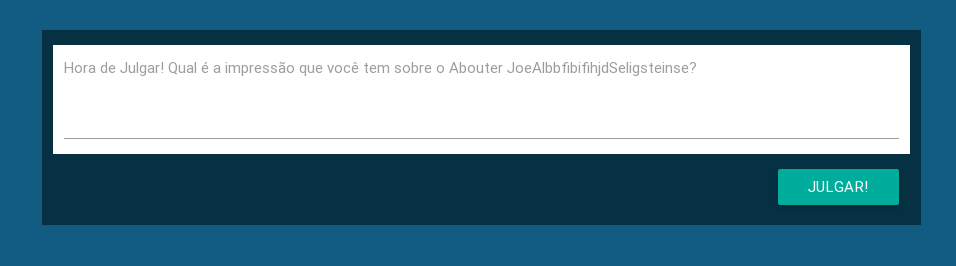
\includegraphics[width=350px, scale=1]{figuras/julgamento_about}
    \caption{About para Julgamento}
    \label{fig:julgamento_about}
\end{figure}

Depois disso, será apresentado um novo usuário para ser julgado.

\subsection{Implementação para Influência Social}
\label{sub:implementacao_influencia_social}
Para a implementação da Influência social, foi criada a prateleira de troféus, mostrando
ao usuário tudo aquilo que ele conquistou na plataforma. Então, o primeiro passo é definir quais são
as possíveis medalhas que os usuários podem conquistar. Foram criados dois tipos de medalhas com diferentes
níveis: Criador de Abouts, Julgador de Abouts. Estes são os níveis:

\begin{itemize}
    \item \textit{Medal abouter} - Agora você é um abouter;
    \item \textit{Medal 5 abouts} - 5 Abouts Escritos;
    \item \textit{Medal 20 abouts} - 20 Abouts Escritos;
    \item \textit{Medal 100 abouts} - 100 Abouts Escritos;
    \item \textit{Medal 1000 abouts} - 1000 Abouts Escritos;
    \item \textit{Medal 5 judge} - 5 Abouts Julgados;
    \item \textit{Medal 100 judge} - 100 Abouts Julgados;
    \item \textit{Medal 1000 judge} - 1000 Abouts Julgados;
    \item \textit{Medal 5000 judge} - 5000 Abouts Julgados;
    \item \textit{Medal 10000 judge} - 10000 Abouts Julgados;
\end{itemize}

Assim, sempre que o usuário alcança essas metas, o sistema apresenta para ele uma sequência de medalhas
conquistadas.

Antes disso, na página do usuário, logo depois do login, existe uma funcionalidade onde este entra para visualizar toda a sua prateleira.
Existe uma medalha que o usuário já tem no momento que está na rede: a \textit{Medal Abouter},
que indica que este agora é um Abouter - nomenclatura utilizada para denominar os usuários da rede social -,
e está na plataforma.
Assim, o usuário necessita apenas clicar no botão apresentado na figura \ref{fig:about_trofeus}.
Quando ele clicar neste botão, o painel irá abrir na parte inferior da aplicação, apresentando todas
as medalhas que este usuário possui, assim como na figura \ref{fig:show_trofeus}.

\begin{figure}[h]
    \centering
    
\includegraphics[width=150px, scale=1]{figuras/about_trofeus}
    \caption{Botão para listar Troféus}
    \label{fig:about_trofeus}
\end{figure}


\begin{figure}[h]
    \centering
    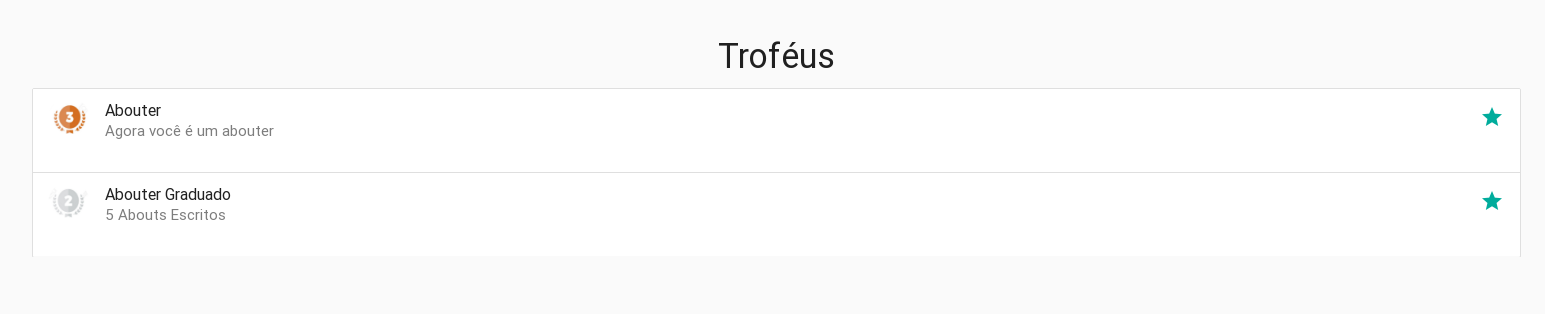
\includegraphics[width=450px, scale=1]{figuras/show_trofeus}
    \caption{Prateleira de Troféus}
    \label{fig:show_trofeus}
\end{figure}

Outra técnica aplicada foi o orgulho social, apresentando para qualquer usuário todas as impressões que os demais
tem sobre ele. Esta técnica é extremamente importante para a que o usuário se mantenha motivado
na fase do dia a dia. Pois gera no usuário uma vontade de se tornar influente através dos abouts feitos em sua
timeline. Caso os abouts sejam positivos, os usuários vão olhar este perfil com bons olhos e começará
a ser mais influente na comunidade que atua.
Os abouts do perfil podem ser vistos na figura \ref{fig:show_profile}.

\begin{figure}[h]
    \centering
    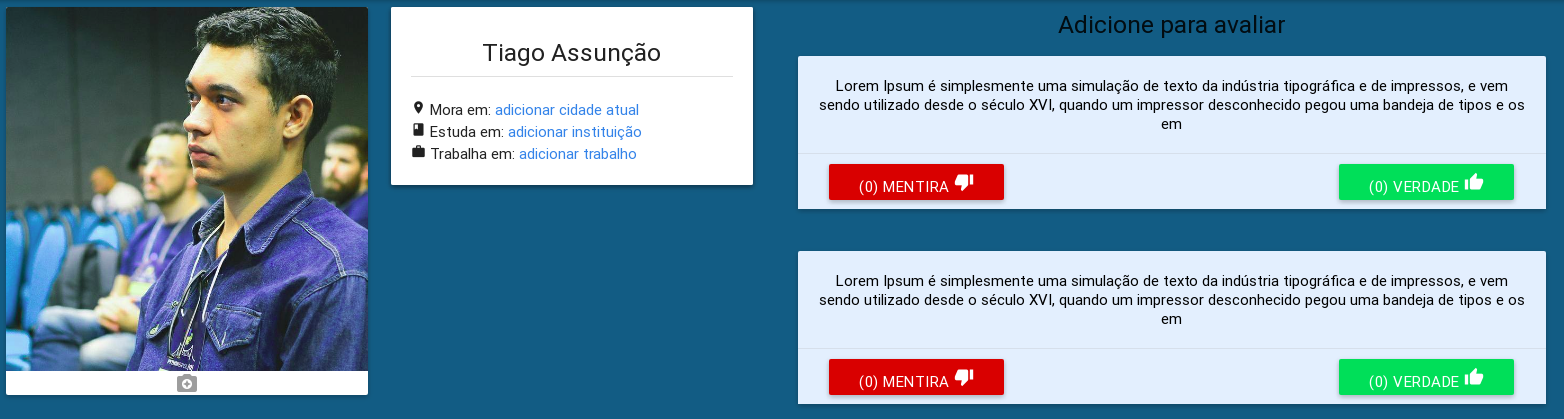
\includegraphics[width=450px, scale=1]{figuras/show_profile}
    \caption{Perfil do Usuário com abouts}
    \label{fig:show_profile}
\end{figure}

Essas foram as técnicas utilizadas na motivação básica de Influência Social. As próximas
serão apresentadas na sessão seguinte \ref{sub:implementacao_imprevisibilidade}.

\subsection{Implementação Imprevisibilidade \& Escassez}
\label{sub:implementacao_imprevisibilidade}

Como dito anteriormente, a About em si já é gamificada e possui as motivações básicas Imprevisibilidade \&
Escassez. 
Nesta sessão, iremos evidenciá-las. 

O primeiro ponto, da imprevisibilidade, pode ser visto que o usuário nunca saberá se virão
abouts positivos ou negativos. Além disso, se estes serão votados positivamente ou não. 

Já a escassez se dá nos mesmos objetos, porém de formas diferentes. O usuário está privado
de saber quem escreveu aquele About, até que este seja desbloqueado. Da mesma forma, não exite
nenhuma informação dos votos executados naquele About. O usuário não tem esse tipo de informação.

O usuário também está privado de todo o tipo de informação caso esteja fora da About, o que motiva-o
a querer estar dentro dela, participando e interagindo com a comunidade. Além disso, este é prejudicado
por não  conseguir ver o que todos os demais estão falando e comentando sobre outras pessoas, seja no
ambiente profissional, familiar ou informal da roda de amigos.

\subsection{Objeto para Desenvolvimento e Realização}
\label{sub:objeto_desenvolvimento_e_realizacao}
Para a implementação da motivação básica do Desenvolvimento e Realização foram utilizadas duas técnicas.
Tanto quanto para a pontuação do usuário, quanto para a barra de progresso. Então foi criado um padrão de pontuação para
o usuário. Assim, como a barra de progresso utilizando níveis.

Para a pontuação, um usuário ganha uma quantidade de pontos X a cada About que ele escreve ou julga.
Para esta pontuação, existe uma base para iniciar a contagem. Exemplo: se X vale 10 pontos, a cada About escrito e
julgado, ele ganha 10 e 1 pontos respectivamente. 
Porém, existe um sistema de incentivo para que o usuário entre na plataforma todos os dias. O valor de X para a pontuação
é incrementado em 10 cada dia consecutivo que este interage com a plataforma. Assim, se o usuário escreve no dia 1 e no dia 2,
neste segundo dia, o valor de X vale 20, no dia 3, irá valer 40. E este incremento só irá ser finalizado
caso o usuário não faça nenhuma interação durante aquele dia.

Estes pontos são utilizados também para o esquema de níveis da aplicação. O usuário conquista níveis maiores
conforme ganha pontos. Ao todo são 23 níveis, estes serão apresentados a seguir:

\begin{itemize}
    \begin{multicols}{2}
        \item 0: 0;
        \item 1: 240;
        \item 2: 600;
        \item 3: 1080;
        \item 4: 1680;
        \item 5: 2300;
        \item 6: 2940;
        \item 7: 3600;
        \item 8: 4280;
        \item 9: 5080;
        \item 10: 5900;
        \item 11: 6740;
        \item 12: 7640;
        \item 13: 8865;
        \item 14: 10115;
        \item 15: 11390;
        \item 16: 12690;
        \item 17: 14015;
        \item 18: 15415;
        \item 19: 16905;
        \item 20: 20155;
        \item 21: 22155;
        \item 22: 24405;
        \item 23: 26905;
        \item 24: 28905;
        \item 25: 31000.
    \end{multicols}
\end{itemize}

Dessa forma, sempre que o usuário utiliza a plataforma fazendo abouts ou julgando, ele adquire pontos,
e sobe de níveis - que são apresentados aos usuários.
Veja a figura \ref{fig:niveis}.

\begin{figure}[h]
    \centering
    
\includegraphics[width=450px, scale=1]{figuras/niveis2}
    \caption{Nível do Usuário}
    \label{fig:niveis}
\end{figure}

Sendo assim, é feita uma apresentação ao usuário sobre em qual nível ele atualmente está, quantos
pontos tem na plataforma e quantos faltam para o próximo nível.
Além disso, o níveis se utilizam desta barra de progresso, para informar a caminhada que este ainda
tem até o próximo nível.

\subsection{Implementação para Perda e Rejeição}
\label{sub:implementacao_perda_rejeicao}
Para a implementação de Perda e Rejeição, foi utilizada a técnica \textit{FOMO} \textit{Ponch}. Aqui são utilizados os pontos
do usuário para fazer com que ele se sinta motivado a não deixar a rede social. Assim, como explicado na
sessão \ref{sub:objeto_desenvolvimento_e_realizacao}
existe um sistema de pontuação para criação e votação de abouts. Esta presente técnica trabalha com o fato
do usuário querer ganhar mais e mais pontos.

Como depois de dias consecutivos escrevendo abouts, o usuário acumula bônus de pontos para utilizar na rede
social em si, desta forma, foi executada a implementação para que quando o usuário não interaja por um dia, ele
perda todos esses números.

A seguir, na figura \ref{fig:mensagem_perda}, está a implementação para a execução desta técnica.

\begin{figure}[h]
    \centering
    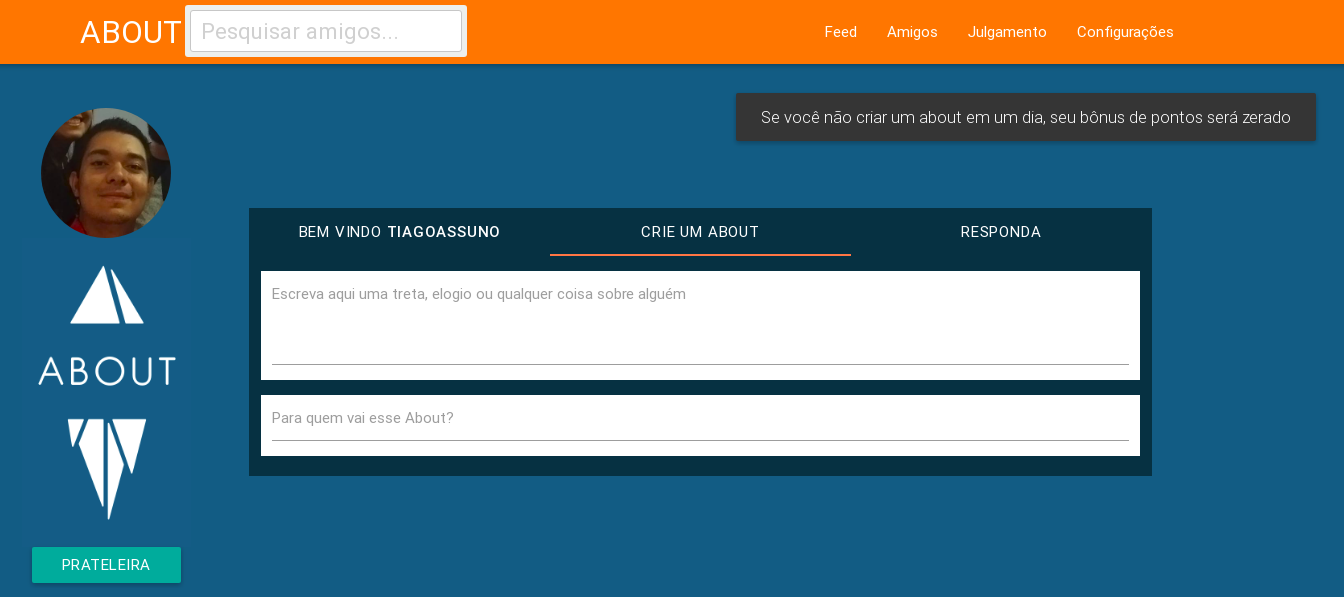
\includegraphics[width=450px, scale=1]{figuras/mensagem_perda}
    \caption{Mensagem de Perda de Pontos do Usuário}
    \label{fig:mensagem_perda}
\end{figure}

Assim, com essas mensagens que podem ser vistas para o usuário no canto superior esquerdo,
o usuário se informa de suas limitações nas questões dos pontos, motivando-se a buscar
sempre estar entrando na rede social About para não perder o bônus.
